\FloatBarrier
\subsection{Kurvenauswertung}



%T_high I_low U_längs
\begin{figure}
\label{}
\centering
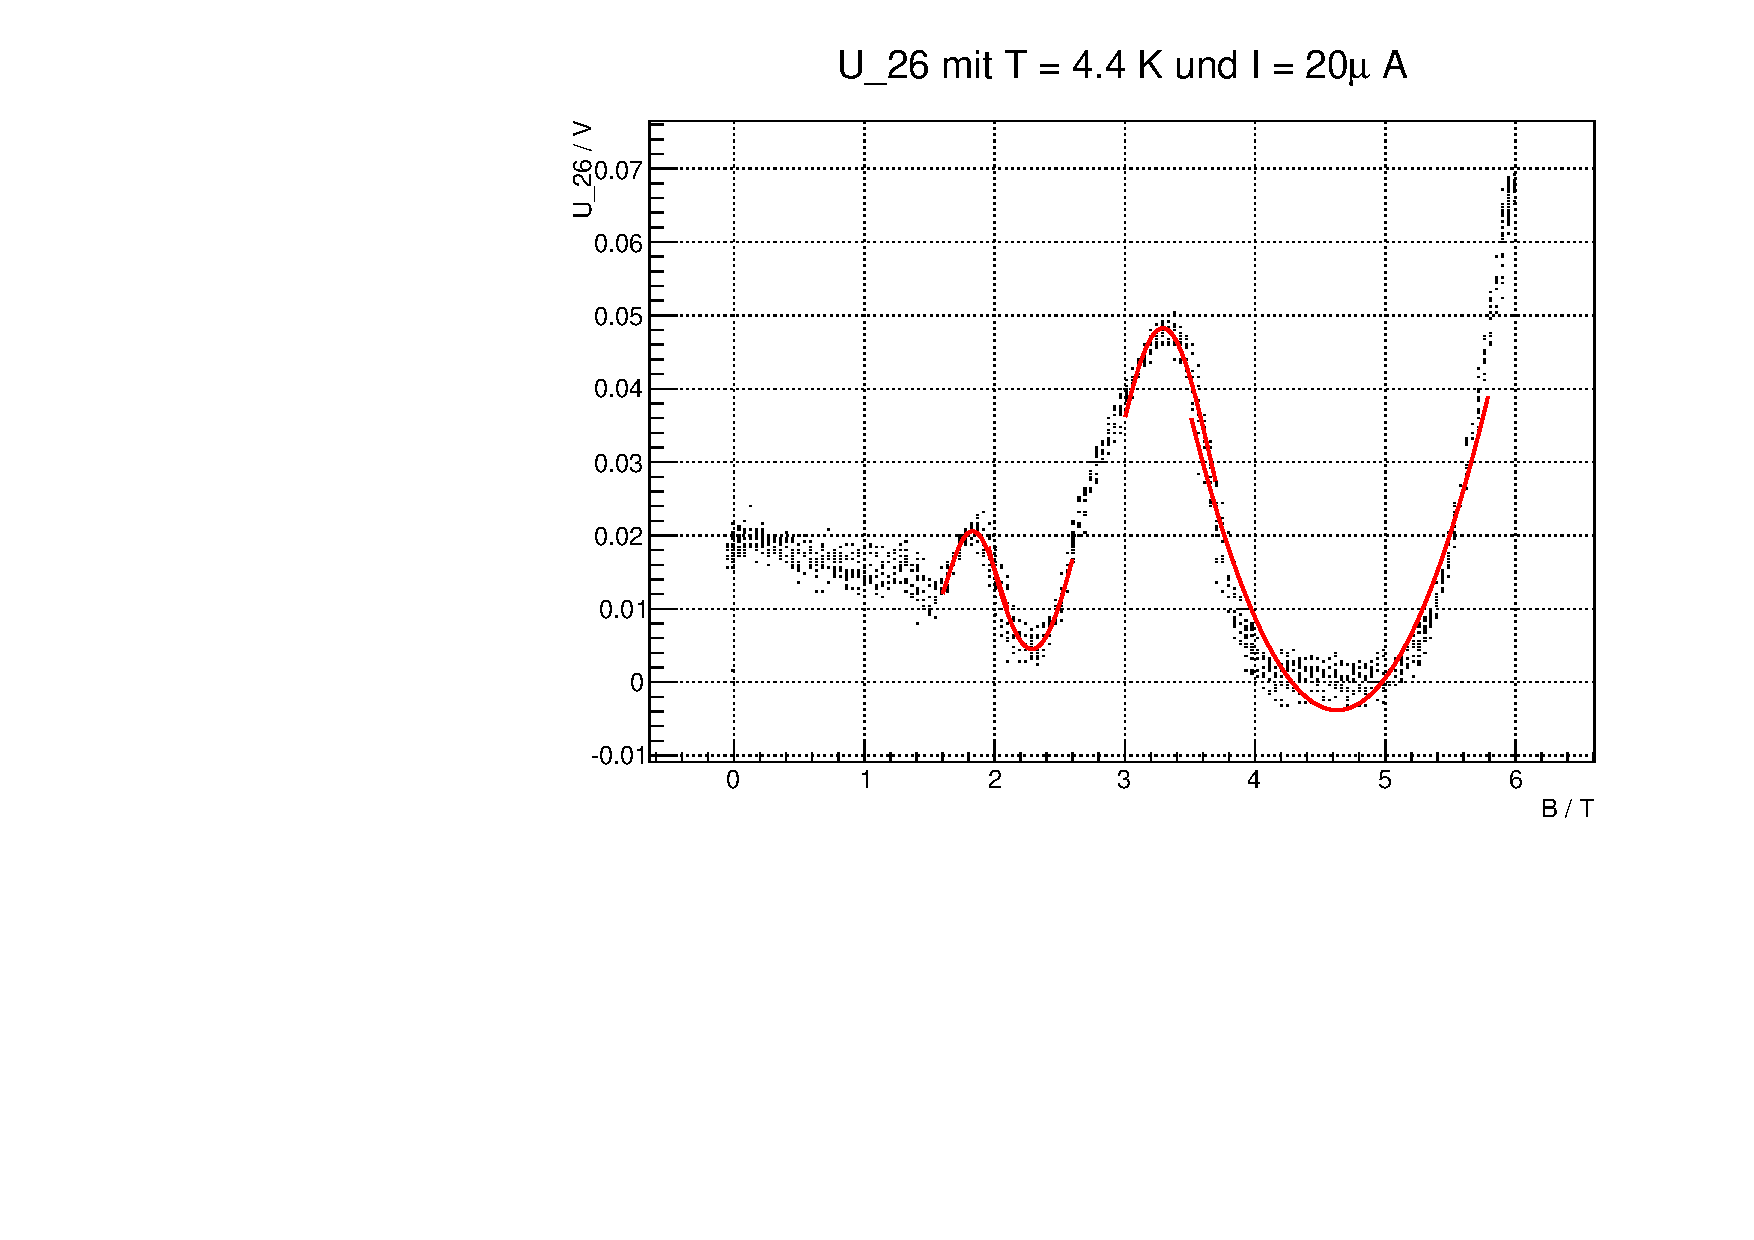
\includegraphics[scale = 0.5]{../plots/U_26_20muA_4400mK.pdf}
\caption{$\text{V}_x$ für I=20 $\mu$A und T=4.4 K}
\end{figure}

%T_high I_high U_längs
\begin{figure}
\label{}
\centering
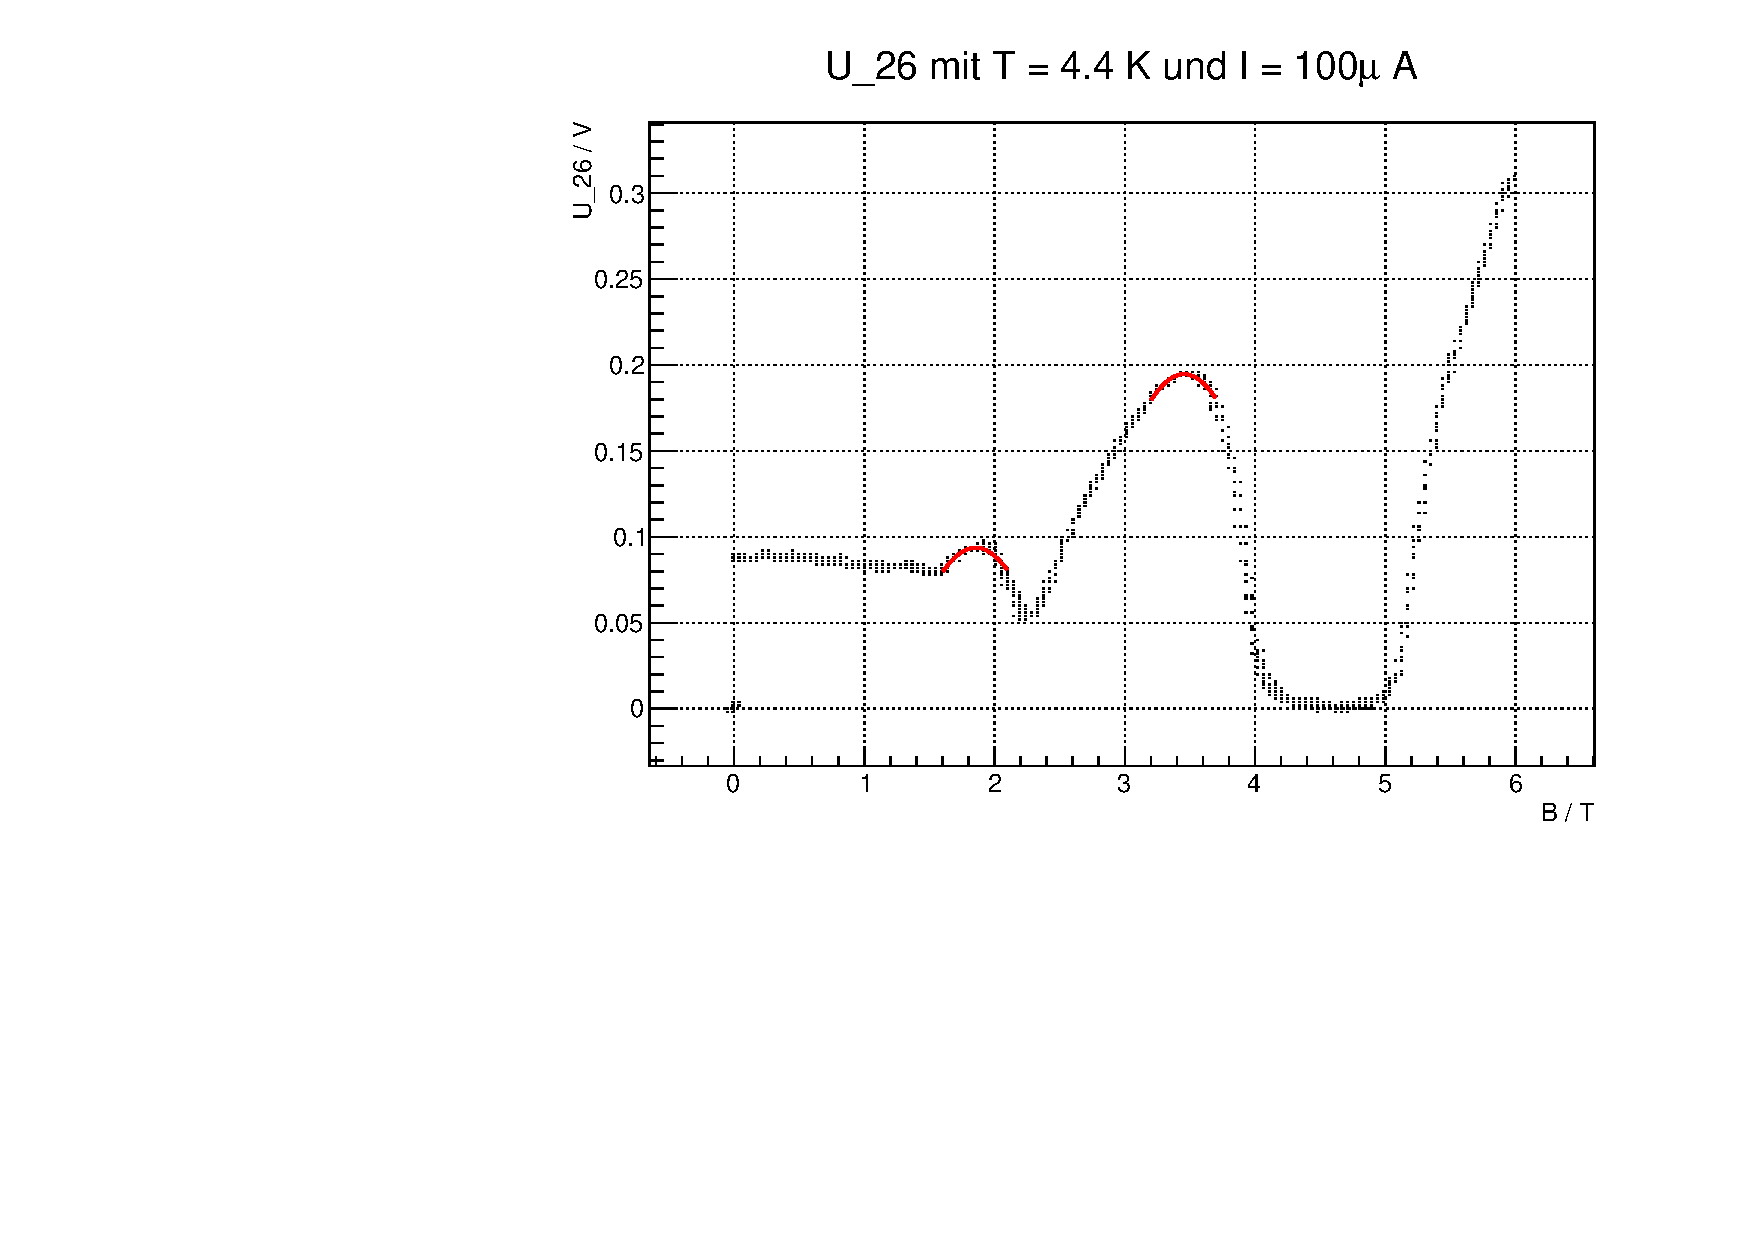
\includegraphics[scale = 0.5]{../plots/U_26_100muA_4400mK.pdf}
\caption{$\text{V}_x$ für I=100 $\mu$A und T=4.4 K}
\end{figure}

%missing
%%T_low I_low U_längs
%\begin{figure}
%\label{}
%\centering
%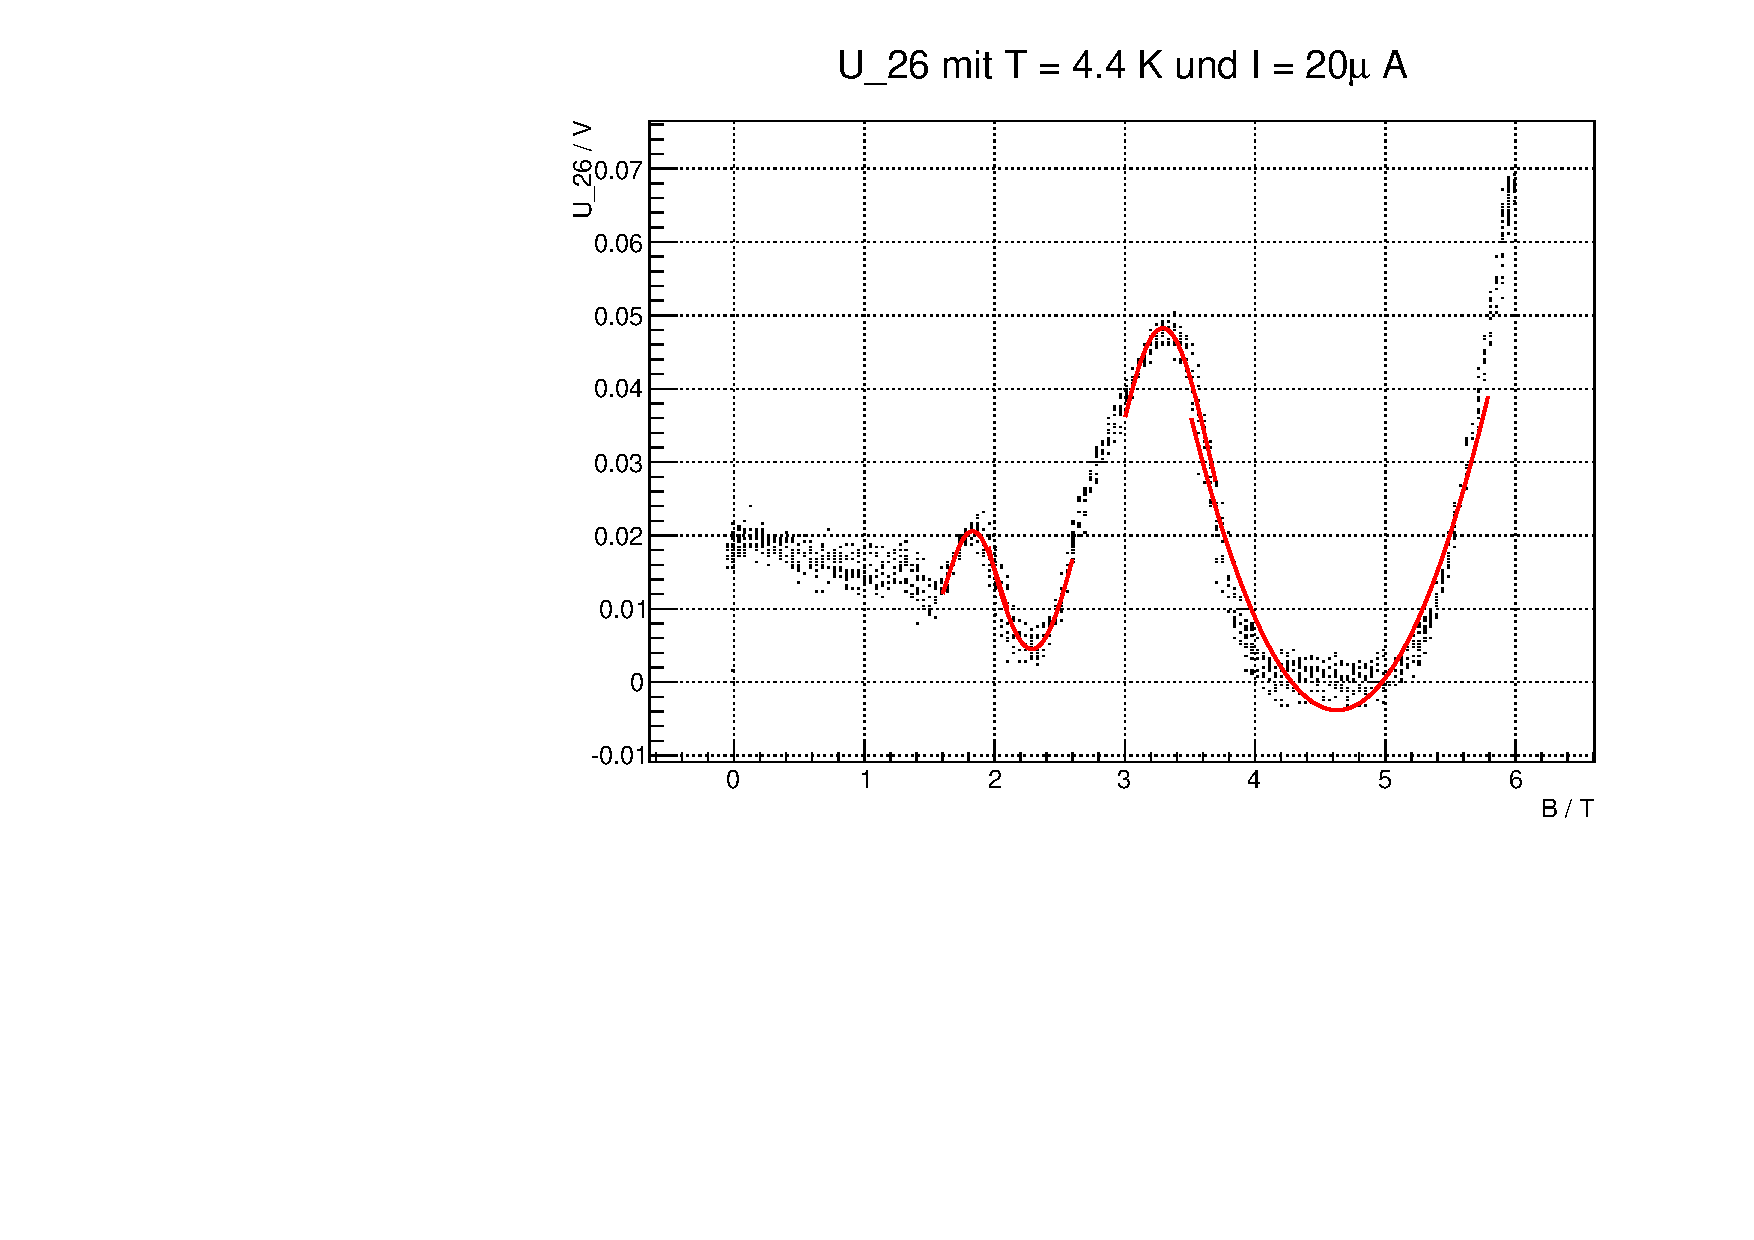
\includegraphics[scale = 0.5]{../plots/U_26_20muA_4400mK.pdf}
%\caption{}
%\end{figure}

%T_low I_high U_längs
\begin{figure}
\label{}
\centering
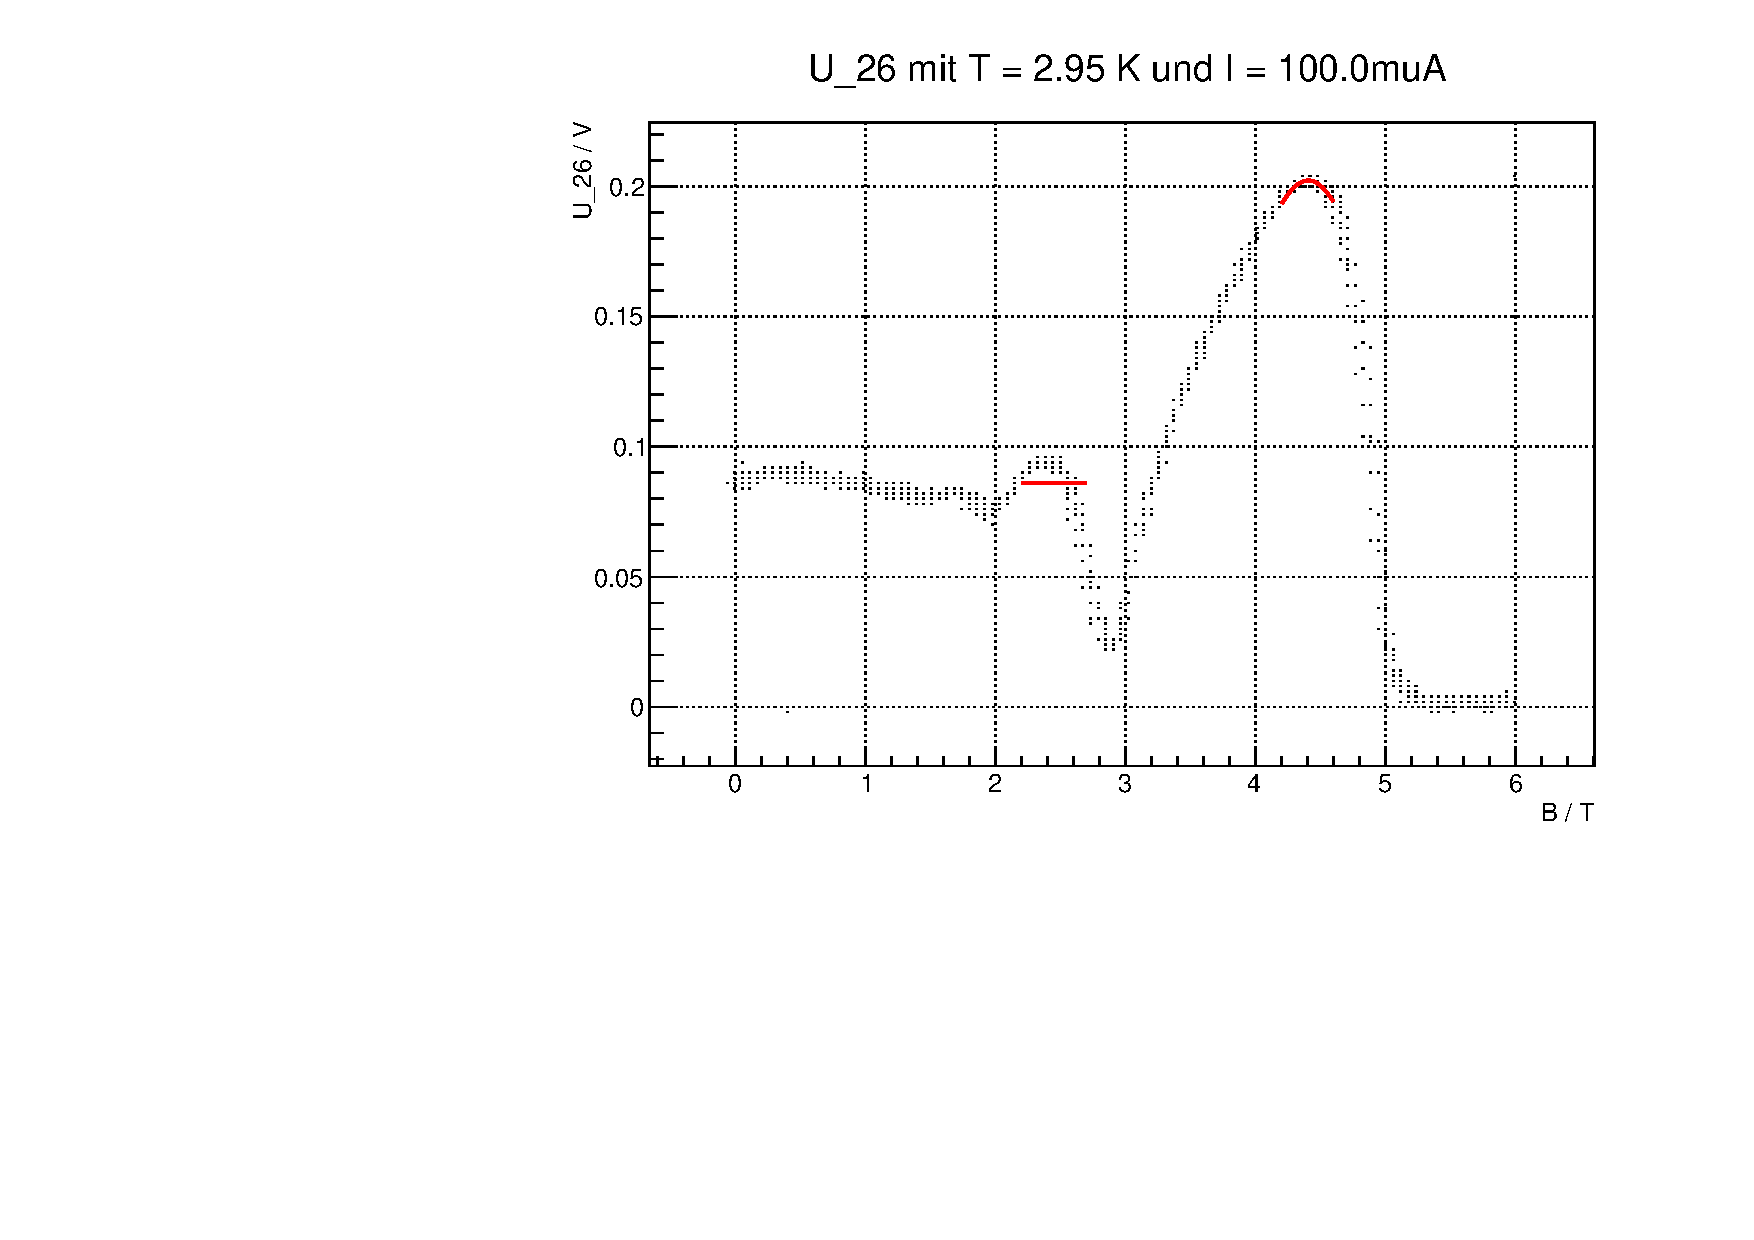
\includegraphics[scale = 0.5]{../plots/U_26_100muA_2950mK.pdf}
\caption{$\text{V}_x$ für I=100 $\mu$A und T=2.95 K}
\end{figure}


%T_high I_low U_hall
\begin{figure}
\label{}
\centering
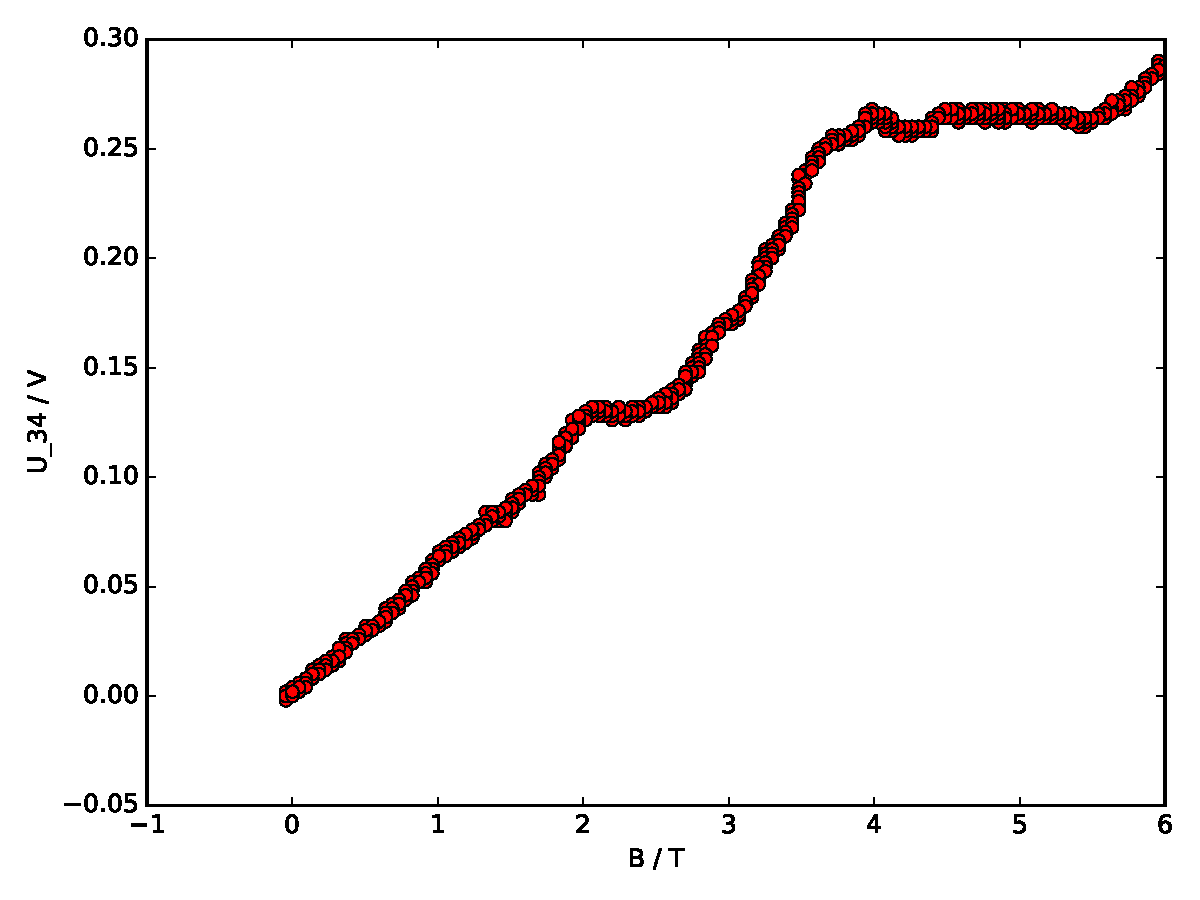
\includegraphics[scale = 0.5]{../plots/U_34_20muA_4100mK.pdf}
\caption{$\text{V}_H$ für I=20 $\mu$A und T=4.1 K}
\end{figure}

%T_high I_high U_hall
\begin{figure}
\label{}
\centering
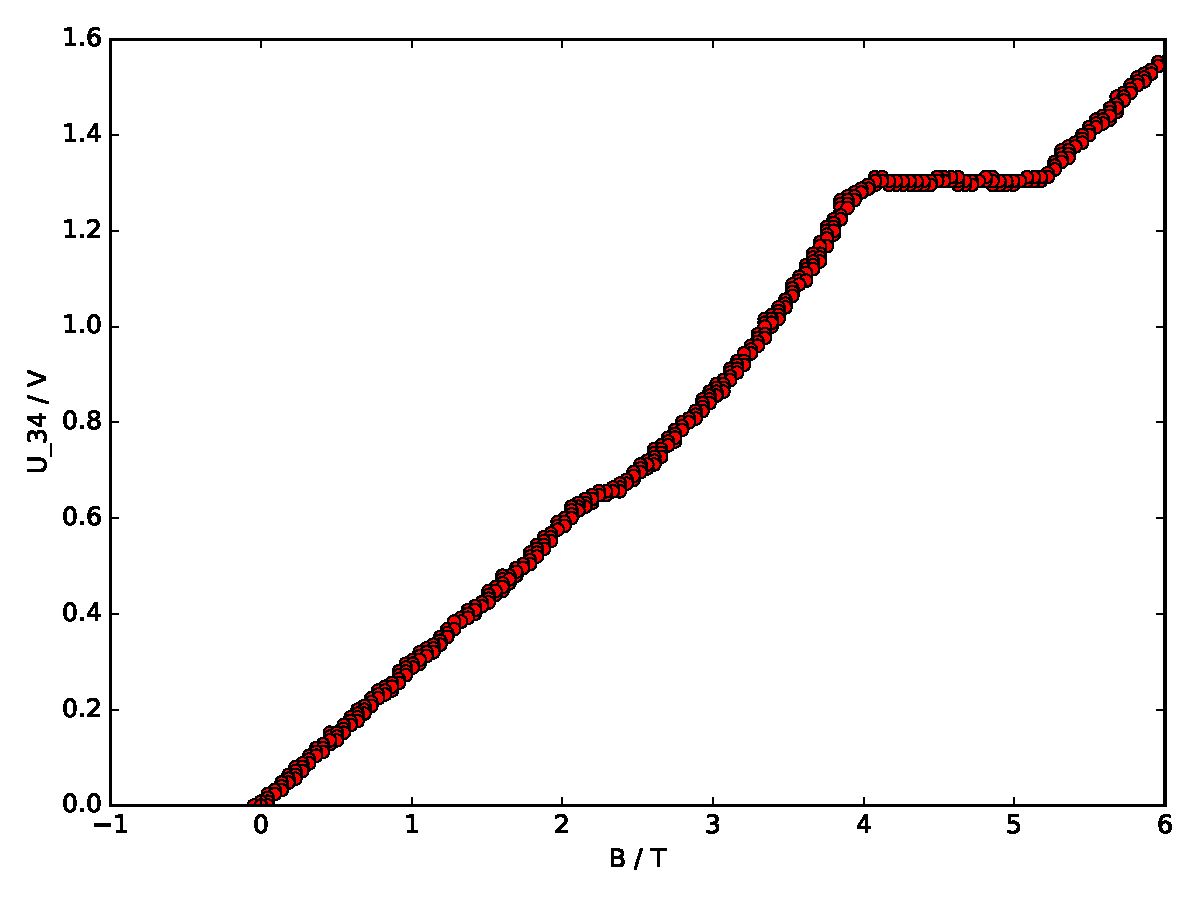
\includegraphics[scale = 0.5]{../plots/U_34_100muA_4400mK.pdf}
\caption{$\text{V}_H$ für I=100 $\mu$A und T=4.4 K}
\end{figure}

%T_low I_low U_hall
\begin{figure}
\label{}
\centering
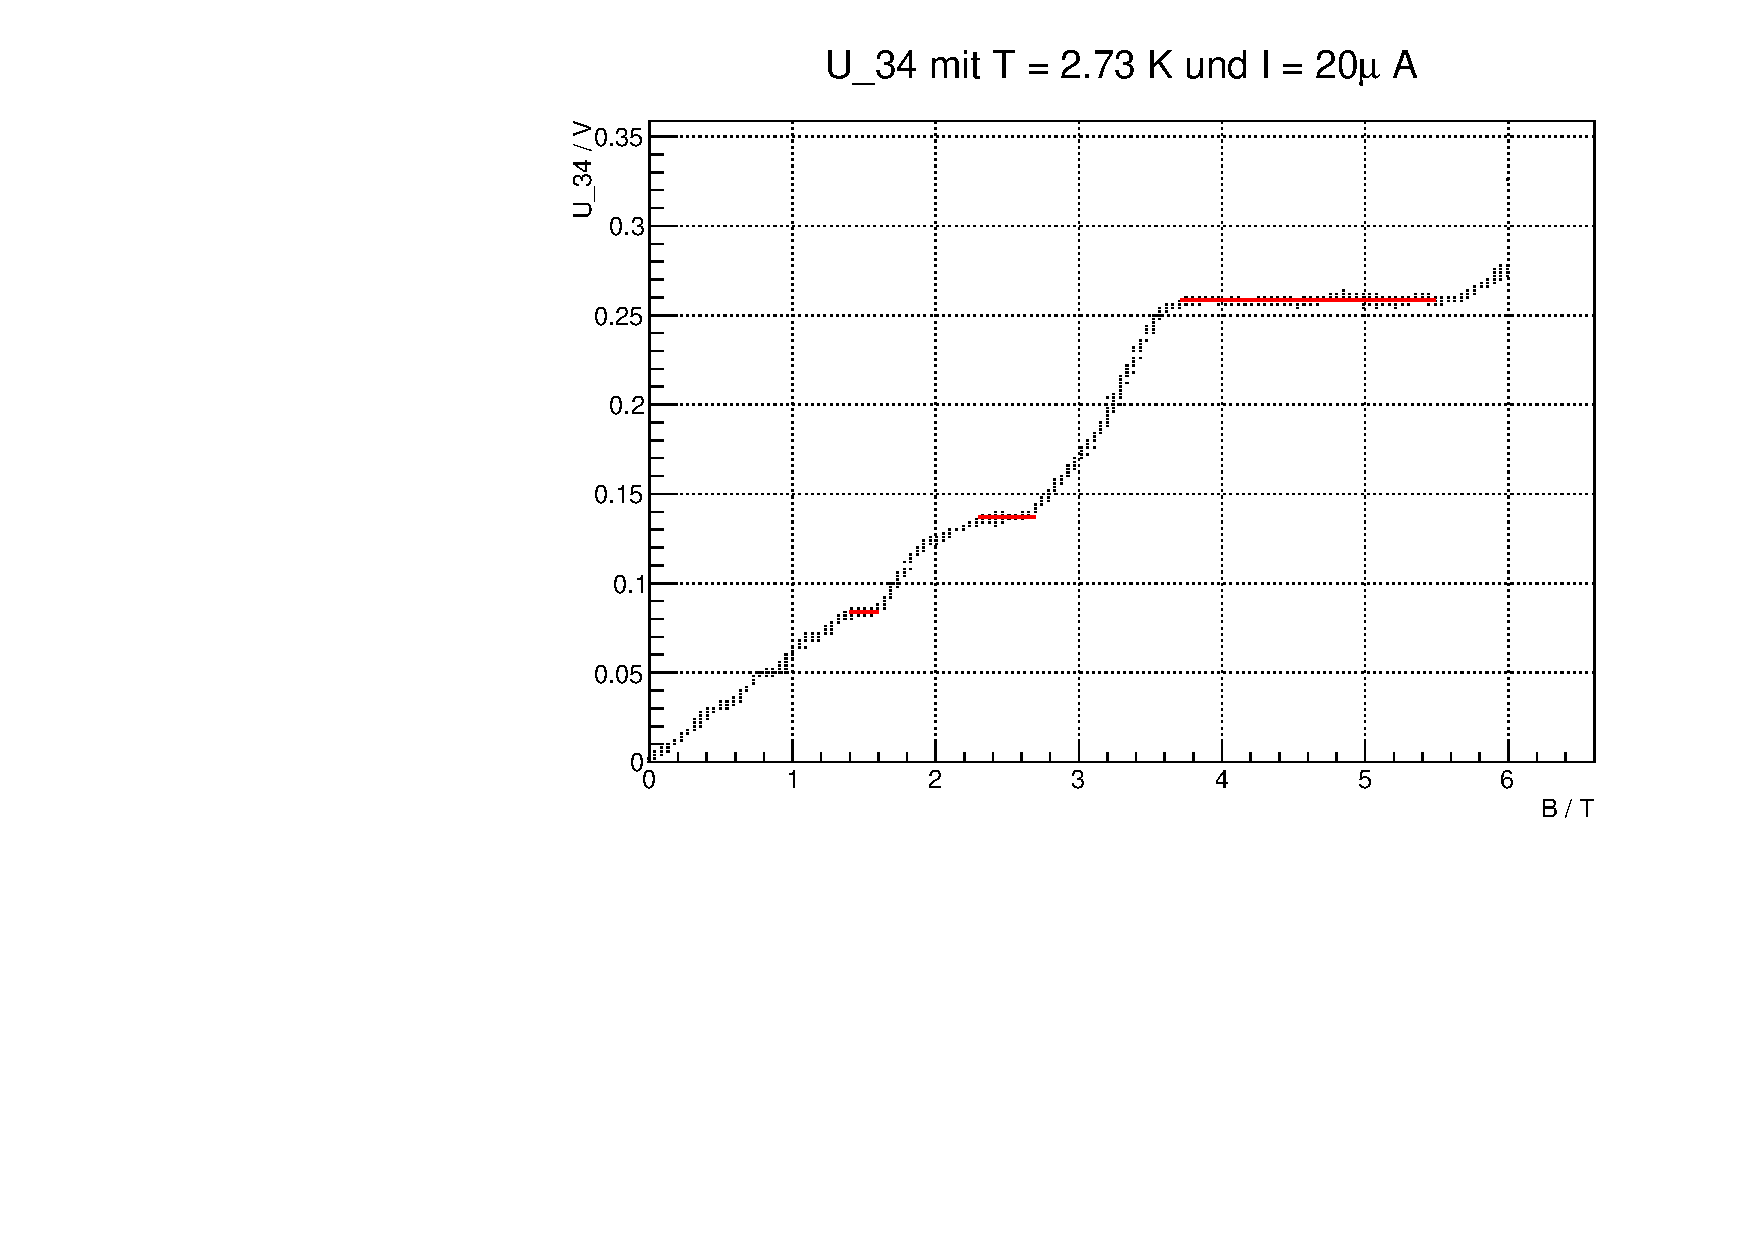
\includegraphics[scale = 0.5]{../plots/U_34_20muA_2730mK.pdf}
\caption{$\text{V}_H$ für I=20 $\mu$A und T=2.73 K}
\end{figure}

%T_low I_high U_hall
\begin{figure}
\label{}
\centering
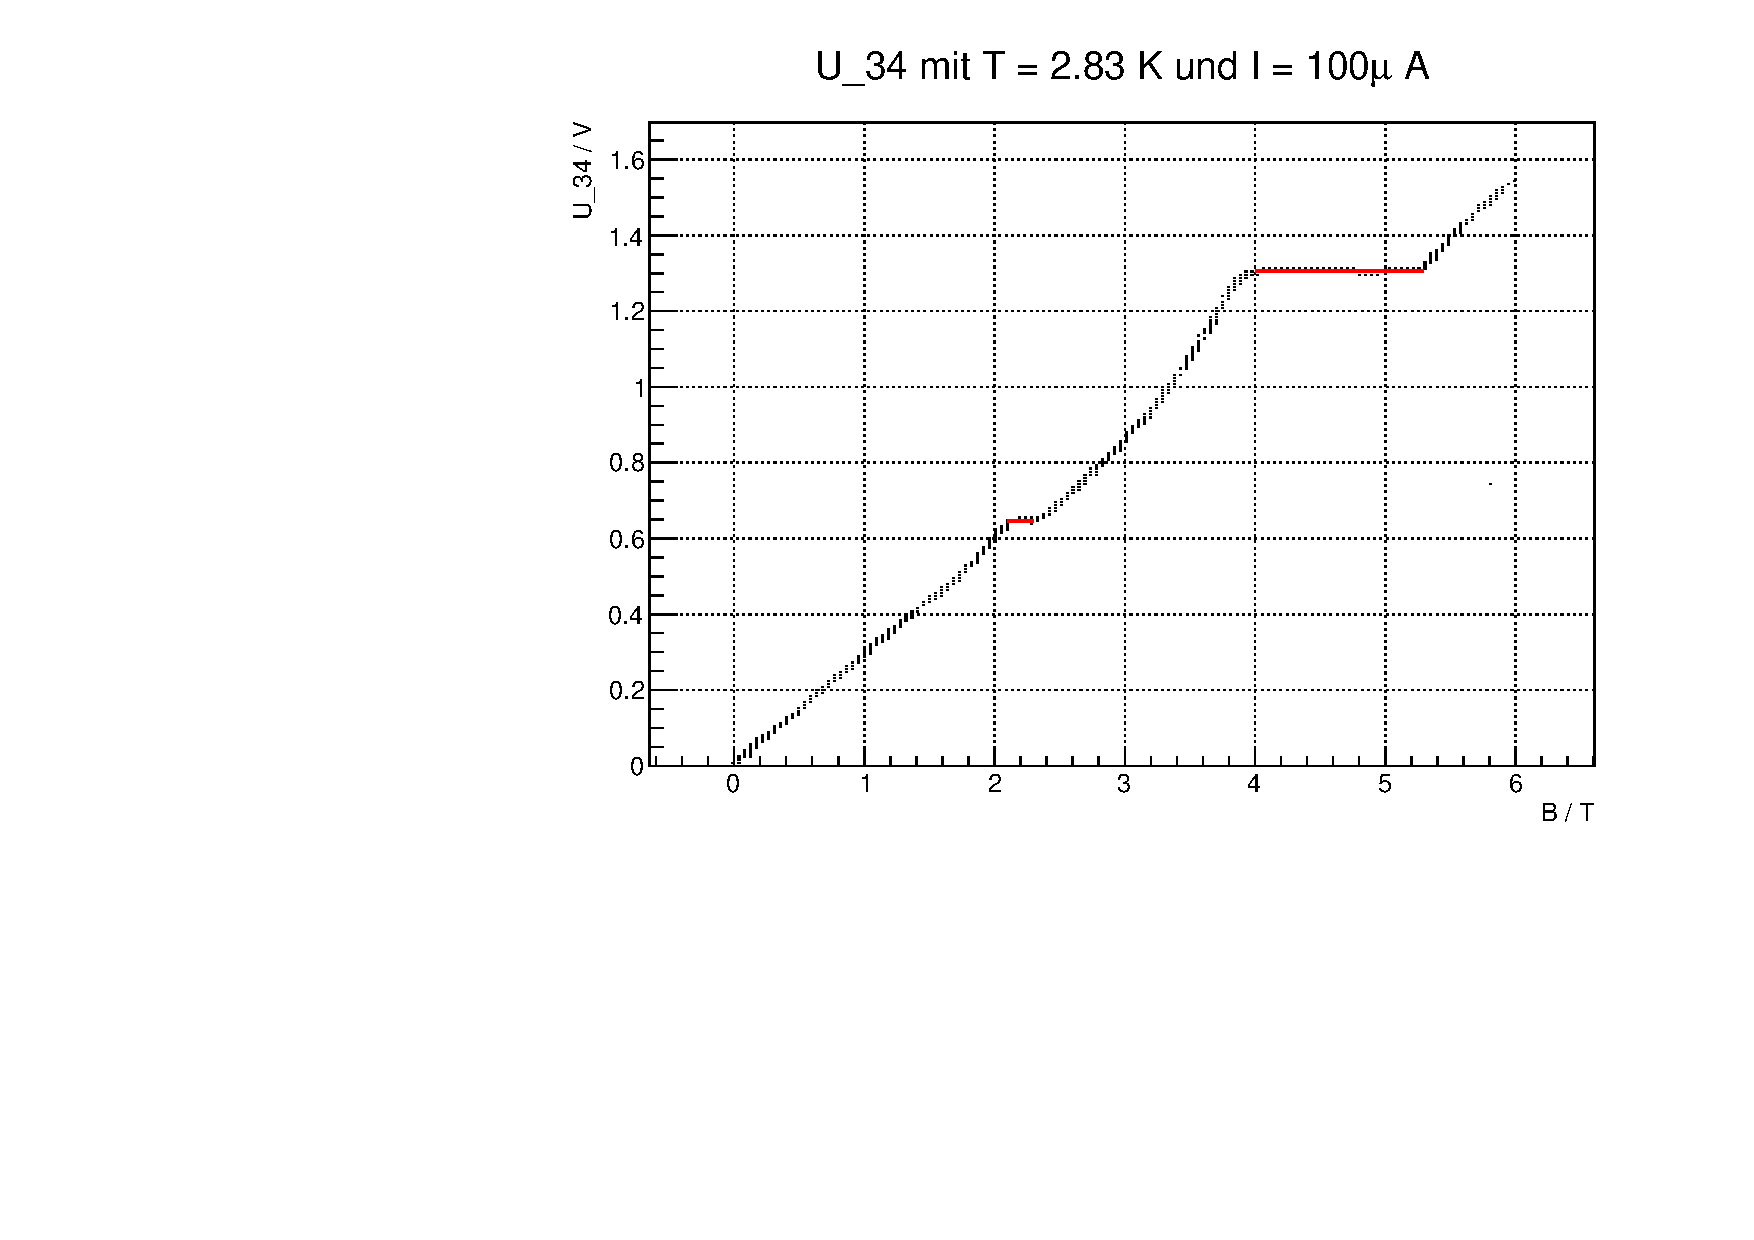
\includegraphics[scale = 0.5]{../plots/U_34_100muA_2830mK.pdf}
\caption{$\text{V}_H$ für I = 100 $\mu$A und T=2.83 K}
\end{figure}


\FloatBarrier


\subsubsection{Längsspannung}

\subsubsection{Hall-Plateaus}

\subsubsection{Ladungsträgerkonzentration}

\subsection{Feinstrukturkonstante}

\subsection{Literaturvergleich}
